\documentclass[ignorenonframetext,]{beamer}
\setbeamertemplate{caption}[numbered]
\setbeamertemplate{caption label separator}{: }
\setbeamercolor{caption name}{fg=normal text.fg}
\beamertemplatenavigationsymbolsempty
\usepackage{lmodern}
\usepackage{amssymb,amsmath}
\usepackage{ifxetex,ifluatex}
\usepackage{fixltx2e} % provides \textsubscript
\ifnum 0\ifxetex 1\fi\ifluatex 1\fi=0 % if pdftex
  \usepackage[T1]{fontenc}
  \usepackage[utf8]{inputenc}
\else % if luatex or xelatex
  \ifxetex
    \usepackage{mathspec}
  \else
    \usepackage{fontspec}
  \fi
  \defaultfontfeatures{Ligatures=TeX,Scale=MatchLowercase}
\fi
\usetheme[]{CambridgeUS}
\usecolortheme{beaver}
\usefonttheme{structurebold}
% use upquote if available, for straight quotes in verbatim environments
\IfFileExists{upquote.sty}{\usepackage{upquote}}{}
% use microtype if available
\IfFileExists{microtype.sty}{%
\usepackage{microtype}
\UseMicrotypeSet[protrusion]{basicmath} % disable protrusion for tt fonts
}{}
\newif\ifbibliography
\hypersetup{
            pdftitle={A1 - Einleitung und Motivation},
            pdfauthor={Jan-Philipp Kolb},
            pdfborder={0 0 0},
            breaklinks=true}
\urlstyle{same}  % don't use monospace font for urls
\usepackage{graphicx,grffile}
\makeatletter
\def\maxwidth{\ifdim\Gin@nat@width>\linewidth\linewidth\else\Gin@nat@width\fi}
\def\maxheight{\ifdim\Gin@nat@height>\textheight0.8\textheight\else\Gin@nat@height\fi}
\makeatother
% Scale images if necessary, so that they will not overflow the page
% margins by default, and it is still possible to overwrite the defaults
% using explicit options in \includegraphics[width, height, ...]{}
\setkeys{Gin}{width=\maxwidth,height=\maxheight,keepaspectratio}

% Prevent slide breaks in the middle of a paragraph:
\widowpenalties 1 10000
\raggedbottom

\AtBeginPart{
  \let\insertpartnumber\relax
  \let\partname\relax
  \frame{\partpage}
}
\AtBeginSection{
  \ifbibliography
  \else
    \let\insertsectionnumber\relax
    \let\sectionname\relax
    \frame{\sectionpage}
  \fi
}
\AtBeginSubsection{
  \let\insertsubsectionnumber\relax
  \let\subsectionname\relax
  \frame{\subsectionpage}
}

\setlength{\parindent}{0pt}
\setlength{\parskip}{6pt plus 2pt minus 1pt}
\setlength{\emergencystretch}{3em}  % prevent overfull lines
\providecommand{\tightlist}{%
  \setlength{\itemsep}{0pt}\setlength{\parskip}{0pt}}
\setcounter{secnumdepth}{0}

\title{A1 - Einleitung und Motivation}
\author{Jan-Philipp Kolb}
\date{22 Oktober 2018}

\begin{document}
\frame{\titlepage}

\begin{frame}

\end{frame}

\begin{frame}{}


\includegraphics{figure/BildRatSWDBericht.png}

\end{frame}

\begin{frame}{\href{http://blog.revolutionanalytics.com/2012/07/making-beautiful-maps-in-r-with-ggmap.html}{Worum
geht es?}}

\begin{block}{Weine probieren im Napa Valley?}

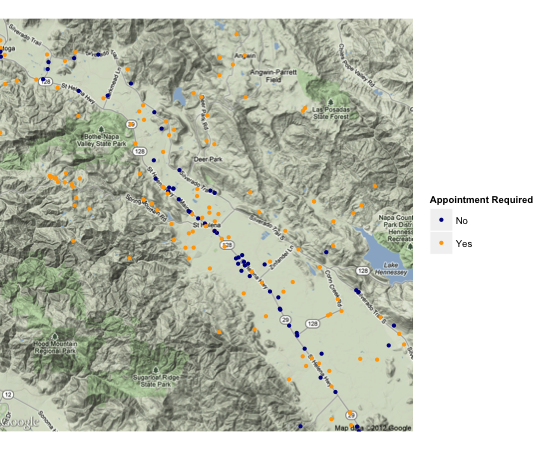
\includegraphics{figure/Wine_nappa.png}

\end{block}

\end{frame}

\begin{frame}{Ziel dieses Kurses}

\begin{block}{Vorgestellt wird:}

\begin{itemize}
\tightlist
\item
  Möglichkeiten für den Download, den Import, die Verarbeitung und die
  Visualisierung von Geodaten
\end{itemize}

\begin{itemize}
\item
  Die wichtigsten Programmierschnittstellen (APIs) um die Daten zu
  bekommen
\item
  R-Pakete um diese Daten zu verarbeiten und zu visualisieren
\end{itemize}

\end{block}

\end{frame}

\begin{frame}{Motivation}

\begin{itemize}
\tightlist
\item
  Sekundäranalyse für bestehenden Daten
\item
  Raumbezug herstellen/nutzen
\item
  Analysepotentiale der Geokodierung vorstellen
\item
  Verbindung von sozial- mit raumwissenschaftlichen Daten
\end{itemize}

\end{frame}

\begin{frame}{\href{http://de.slideshare.net/rheimann04/big-social-data-the-spatial-turn-in-big-data}{Laws
of Spatial Sience}}

\href{https://en.wikipedia.org/wiki/Tobler's_first_law_of_geography}{Tobler's
law}

\begin{quote}
everything is related to everything else, but near things are more
related than distant things.
\end{quote}

\end{frame}

\begin{frame}{\href{https://de.wikipedia.org/wiki/Spatial_turn}{Spatial
Turn}}

\begin{quote}
Spatial turn is a term used to describe an intellectual movement that
places emphasis on place and space in social science and the humanities.
\end{quote}

\href{https://en.wikipedia.org/wiki/Spatial_turn}{Englisches Wikipedia}

\end{frame}

\begin{frame}{Regional/geographical differences in the perception
of\ldots{}}

\begin{itemize}
\tightlist
\item
  \ldots{} measures to promote climatic change
\item
  \ldots{} big infrastructure projects
\end{itemize}

\end{frame}

\begin{frame}{Ergebnisse des Zensus 2011 zum
\href{https://www.zensus2011.de/SharedDocs/Aktuelles/Ergebnisse/DemografischeGrunddaten.html?nn=3065474}{\textbf{Download}}}


\includegraphics{figure/zensus2011_logo.jpg}

\begin{block}{Gemeindeebene}

\begin{itemize}
\tightlist
\item
  Bevölkerung nach Geschlecht, Altersgruppe, Familienstatus,
  Staatsangehörigkeit und Religion
\end{itemize}

\end{block}

\begin{block}{1 \(\text{km}^2\) Raster}

\begin{itemize}
\tightlist
\item
  Bevölkerung, Leerstandsquote, Wohnfläche und Haushaltsgröße
\end{itemize}

\end{block}

\begin{block}{100 \(\text{m}^2\) Raster}

Bevölkerung

\end{block}

\end{frame}

\begin{frame}{Zensus Ergebnisse}

Beispiel Anteil der Personen aus EU27 Land an Einwohnerzahl pro Gemeinde
in Oberfranken

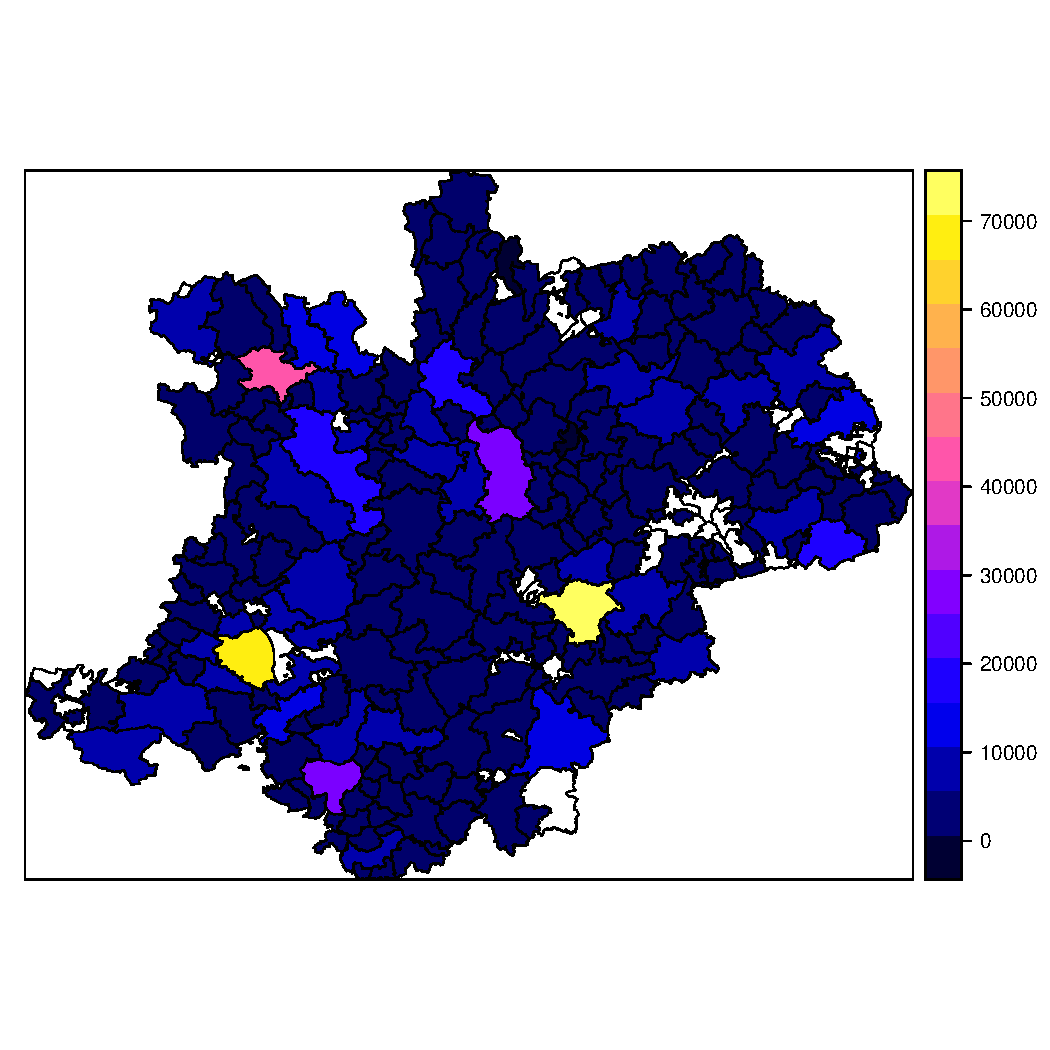
\includegraphics{figure/KRSBamberg_EWZ.pdf}

\end{frame}

\begin{frame}{Motivation - Warum die Darstellung in Karten}

\begin{itemize}
\item
  Darstellung in Karten ermöglicht besseres Verständnis bspw.
  sozialwissenschaftlicher Phänomene.
\item
  Attraktiver Output
\item
  Durch die INSPIRE Richtlinie und \emph{Collaborative Mapping} wächst
  der verfügbare Bestand an Geodaten.
\item
  Daten sind oft frei verfügbar im Internet (z.B. durch die Nutzung von
  APIs)
\item
  Die Daten sind allerdings oft wenig oder gar nicht strukturiert (z.B.
  Internet Dokumente), heterogen und
\item
  meistens nicht für die Nutzung zur räumlichen Visualisierung
  vorgesehen, beinhalten aber implizit geographische Informationen (Web
  2.0)
\item
  Oftmals sind wenig oder keine Metadaten vorhanden
\end{itemize}

\end{frame}

\begin{frame}{\href{https://wiki.openstreetmap.org/wiki/Tags}{Openstreetmap
Tags}}


\includegraphics{figure/osm_tag.png}

\end{frame}

\begin{frame}{Openstreetmap Projekt}

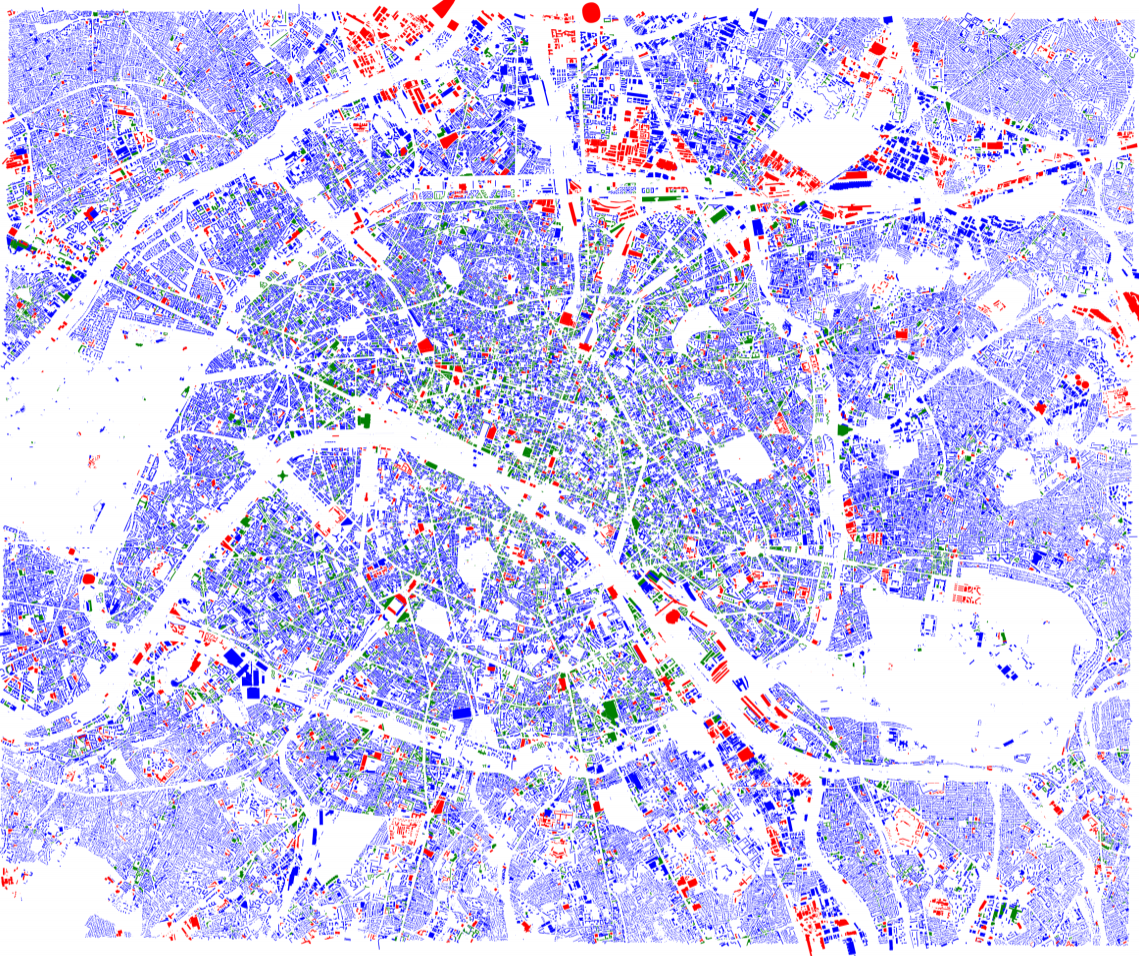
\includegraphics{figure/Buldings_Paris.PNG}

\end{frame}

\begin{frame}{Was ist das Ziel - Straßen in Berlin}

Dargestellt werden OpenStreetMap Daten, die mit der Overpass API
heruntergeladen wurden.

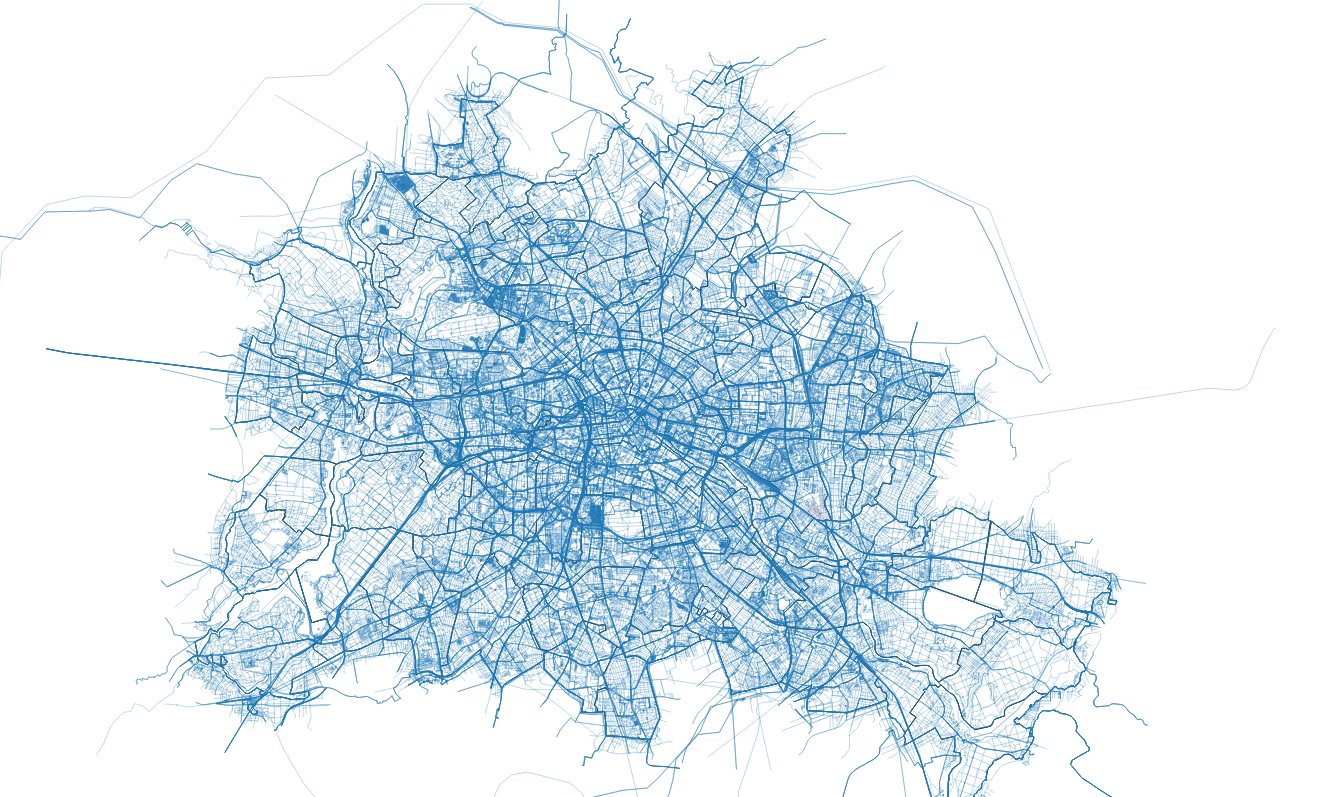
\includegraphics{figure/streets_Berlin2.png}

\end{frame}

\begin{frame}{Global patterns of current and future road infrastructure}

\begin{block}{Study by Johan Meijer, Mark AJ Huijbregts, Kees Schotten,
and Aafke Schipper}

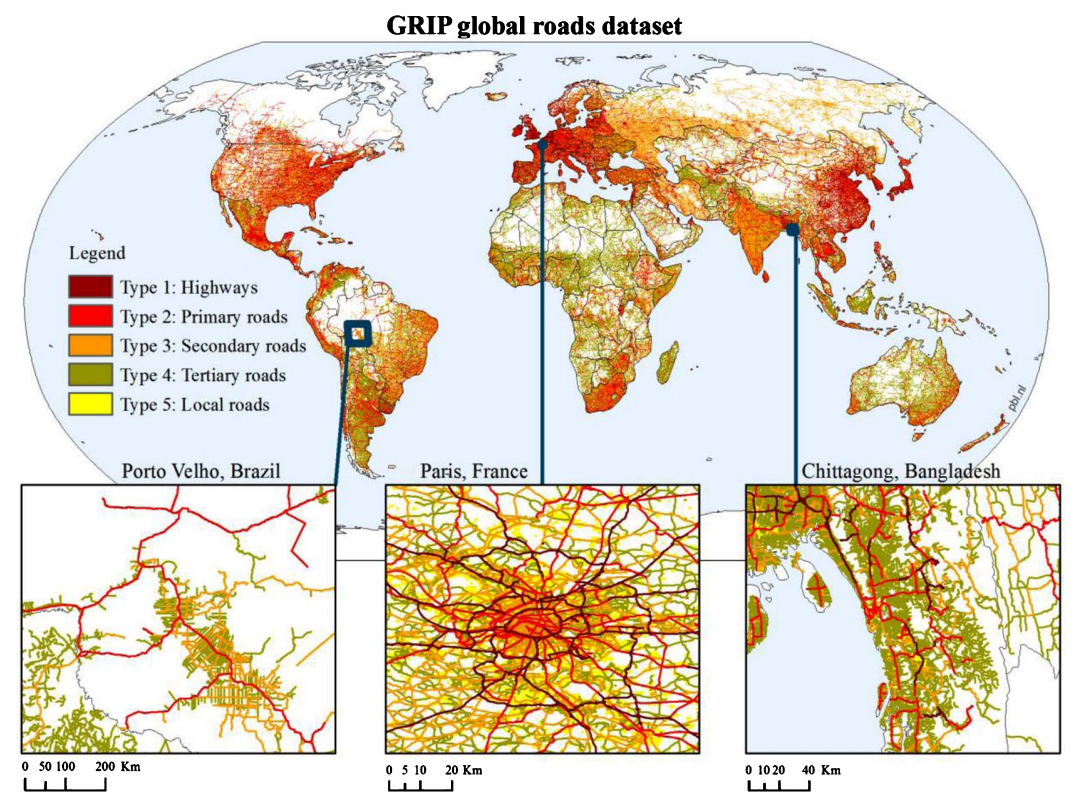
\includegraphics{figure/GRIP_globalroads.PNG}

\end{block}

\end{frame}

\begin{frame}{Links mit Beispielen}

\begin{itemize}
\item
  Shiny App zu
  \href{https://japhilko.shinyapps.io/Choropleths/}{\textbf{Indikatoren}}
  für Europa
\item
  Räumliche Visualisierung in den USA -
  \href{https://rpubs.com/Radcliffe/walmart}{\textbf{Walmarts in den
  USA}}
\item
  \href{http://www.nytimes.com/interactive/2014/09/03/us/the-race-gap-in-americas-police-departments.html?_r=0}{\textbf{Race
  Gap Police USA}} - \href{http://fivethirtyeight.com/}{\textbf{Wahl
  USA}}
\item
  Zeit Artikel zum Zustand der
  \href{http://detektor.fm/digital/datenjournalismus-interaktive-karte-zeigt-marode-deutsche-bahn-bruecken}{\textbf{Eisenbahnbrücken}}
\item
  \href{http://michael-hoerz.de/maps/berlin-bike/}{\textbf{Fahrradunfälle}}
  in Berlin
\item
  \href{http://interaktiv.morgenpost.de/beta-fussballkarte/\#7/51.258/10.756}{\textbf{Verteilung
  Fußballfans}}
\item
  \href{http://news.nationalgeographic.com/news/2014/07/140715-ocean-plastic-debris-trash-pacific-garbage-patch/}{\textbf{Plastiktüten
  im Meer}}
\end{itemize}

\begin{block}{Datenquellen:}

\begin{itemize}
\tightlist
\item
  Datensätze zu
  \href{https://www.pegelonline.wsv.de/gast/start}{\textbf{Pegelständen}}
  in Deutschland
\item
  Viele Datensätze auf \href{http://driven-by-data.net/}{\textbf{driven
  by data}}
\end{itemize}

\end{block}

\begin{block}{Resourcen}

\begin{itemize}
\tightlist
\item
  Andreas Plank -
  \href{http://www.chironomidaeproject.com/fileadmin/downloads/Formeln_in_R.pdf}{\textbf{Grafiken
  und Statistik in R}}
\end{itemize}

\end{block}

\end{frame}

\begin{frame}{Das Openstreetmap Projekt\ldots{}}

\begin{itemize}
\tightlist
\item
  Durch kollaboratives Mapping ist eine riesige Datenmenge zugänglich.
\item
  Viele Menschen tragen jeden Tag Informationen bei.
\item
  \ldots{} ermöglicht Zugang zu Big Data der Geographie.
\item
  Die wachsende Menge an Geodaten wird von Freiwilligen gesammelt oder
  über Crowd-sourcing gewonnen.
\end{itemize}

\end{frame}

\end{document}
